\RequirePackage{lineno}
\documentclass[12pt,a4paper]{article}
\usepackage[T1]{fontenc}
\usepackage{graphicx}
\usepackage{hyperref}
\usepackage{caption}
\usepackage{mathptmx}
\usepackage[absolute,overlay]{textpos}
\usepackage{fancybox}
\usepackage{multirow}
\usepackage[dvipsnames]{xcolor}
\usepackage{amsmath, amsthm, amssymb,amsfonts}
\usepackage{float}
\usepackage{fullpage}
\usepackage{units}
\usepackage{xspace}
\usepackage{caption}
\usepackage{subcaption}

%%% Code to enter C++ code
\usepackage{listings}
\lstset{language=C++,
        basicstyle=\ttfamily,
        keywordstyle=\color{blue}\ttfamily,
        stringstyle=\color{red}\ttfamily,
        commentstyle=\color{green}\ttfamily,
        morecomment=[l][\color{magenta}]{\#}
}

\usepackage{hyperref}
\hypersetup{
    colorlinks,
    citecolor=blue,
    filecolor=black,
    linkcolor=black,
    urlcolor=black
}

\author{Robert Kralik\\\small{University of Sussex}}
\title{NOvA Test Beam detector calibration\\ \vspace*{5mm}
\Large{Technical Note}}
\date{\today}

\begin{document}
\maketitle
\begin{abstract}
What is this about and what will I describe in here
\end{abstract}
\tableofcontents
\newpage

\section{Introduction}
Why is Test Beam?
"The idea, as with any test beam experiment, is to expose a detector to a beam of very well-characterized particles, so that we can improve our understanding our how the detector responds to such particles. We make use of upstream detectors to collect data on the beam particles before they interact in the NOvA detector. For example, we will be able to see what a 1 GeV proton actually looks like in our detector, without having to simulate it, and we can test how well we would have reconstructed the energy using our existing techniques. We may find we are able to make improvements to our tools to better match what we see in the detector with how reconstruct it. Or we may find we already do a pretty good job. Either way, with a full cross-comparison like this, we can be more confident in our analysis of the data and reduce the level of uncertainty we consider are associated with the relevant measured quantities. Ultimately, the aim will be to reduce the level of uncertainty on the neutrino oscillation analyses and to make even better, more accurate measurements of the Standard Model."%[https://cdcvs.fnal.gov/redmine/projects/novatestbeam/wiki/Introduction_to_Test_Beam_for_Analyzers]
Why is Test Beam calibration done:
\begin{itemize}
\item To be able to directly compare TB to the standard detectors
\item To be able to verify our calibration procedures using TB data
\item To compare currently used energy scales to data and understand if we can use TB data for absolute energy scale in all NOvA detectors
\end{itemize}

Only considering improvement in the calibration systematic uncertainty, the NOvA Test Beam program can reduce the overal systematic uncertainty for the main NOvA measurements by about 10\% [docdb:33012] (talk also contains a list of other talks on impact of TB in different NOvA areas).

Also use information from:
\begin{itemize}
\item NOvA Test Beam Technical Statement of Work
\item NOvA Test Beam program (paper for DOE) [docdb:25074]
\item NOvA Test Beam task force report [docdb:15750]
\item Overview presentation of NOvA Test Beam [docdb:20495]
\item Test Beam support document [docdb:22172]
\item NOvA Test Beam program proceedings [docdb:55808]
\end{itemize}

Mike's proceedings from ICHEP 2020 \cite{WallbankProceedingsICHEP2020}.

\section{Overview of Test Beam detector}
What is Test Beam, how does the detector and beamline look like.
What are the main differences between the NOvA standard detectors and the Test Beam detector?
Placed in MC7b together with a beamline instrumentation (no need to describe beamline).
Get a picture of Test Beam.

\subsubsection*{General parameters}
Smaller version of the standard NOvA detectors  made up of 2 vertical and 2 horizontal modules, compared to XxY, or XxY for ND and FD respectively.
" This detector is identical in every way to the Near and Far Detectors but is scaled down, similar to how the Near Detector is a scaled down version of the Far Detector. It consists of 63 planes, and is constructed as a 2x2 module (c.f. ND is 3x3). The total mass is about 30 tons."%[https://cdcvs.fnal.gov/redmine/projects/novatestbeam/wiki/Introduction_to_Test_Beam_for_Analyzers]
63 planes, 32 vertical and 31 horizontal; 64 cells in a plane (2x32 extrusions), readout out in two 32 cell groups;
FD: maxPlane=900, maxCell=390. ND: maxPlane=220, maxCell=100. TB: maxPlane=63, maxCell=64
Detector block taken from NDOS, which had only 31 planes [docdb:28943], beginning and ending with a vertical plane. During comissioning of Test Beam, glued in a horizontal plane in between the two block. [docdb:29543]

Describe the orientation of axes. What's right and left, what's positive and negative w, which planes are vertical and which horizontal (vertical are even starting at 0 and ending in 62 and horizontal are odd).

Readout for the horizontal planes on the opposite side compared to the standard NOvA detectors (why?). Causing underfilled cells in the middle and top of the detector, until... [docdb:49827]
Describe orientation and readout of the TB detector.
Mention the two surveys and the alignment troubles.

\subsubsection*{Scintillator}
Scintillator oil (5600 gallons in total [from Detector Information wiki]) used from ND+NDOS and spare from Texas in the back of the detector (plus some from Ash River afaik).
Block 0 filled with ND+NDOS scintillator oil kept in the tanker [docdb:37152]. Found out the rest of the scintillator in the tanks in Fermilab is contaminated and unusable [docdb:38349] and used NDOS oil from barells to top off horizontal modules.
Shipped scintillator from Ash River and filled the first 21 planes of Block 1 [docdb:41961]. Last 10 planes filled with the NDOS-drained oil from Texas [docdb:34046 describing Texas oil and docdb:41961 showing final filling state].
Maybe show a plot of response at cell centre and mark the 3 different scintillators.

\begin{figure}[hbtp]
\centering
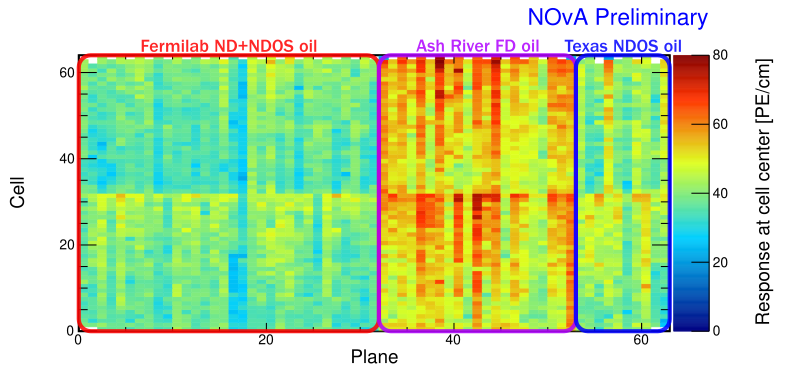
\includegraphics[width=\textwidth]{Plots/TestBeamScintillatorOils.png}
\caption{Fiber brightness file showing the different scintillator oils used in the Test Beam detector}
\end{figure}

\subsubsection*{Readout}
Same readout electronics as in the Far Detector, except for 8 Near Detector Front End Boards, 4 in planes ... (1st quarter of the detector) and another 4 in planes ... (3rd quarter of the detector).
"The Near Detector (ND) and Far Detector (FD) use different versions of the front-end electronics (FEBs, front-end boards), designed to be able to collect data at different rates (the ND is a higher-rate environment than the FD since it is much closer to the beam source). The FD uses FEBv4s (i.e. version 4) and the ND uses FEBv5s. The Test Beam detector uses both in order to be able to make comparisons and validate both versions of the electronics. Most of the FEBs on the Test Beam detector are v4s; of the 126 total, 118 are v4 and 8 are v5."%[https://cdcvs.fnal.gov/redmine/projects/novatestbeam/wiki/Introduction_to_Test_Beam_for_Analyzers]

\subsubsection*{Environment}
Placed in the Fermilab Test Beam Facility with no overburden. Describe environmental controls, temperature dependence etc. Maybe add plots from environmental control (temperature differences etc.) with descriptions of where were the readings taken.


\section{The NOvA calibration}
Describe the NOvA calibration procedure in general. Describe the benefit of NOvA Test Beam and differences.

\begin{figure}[hbtp]
\centering
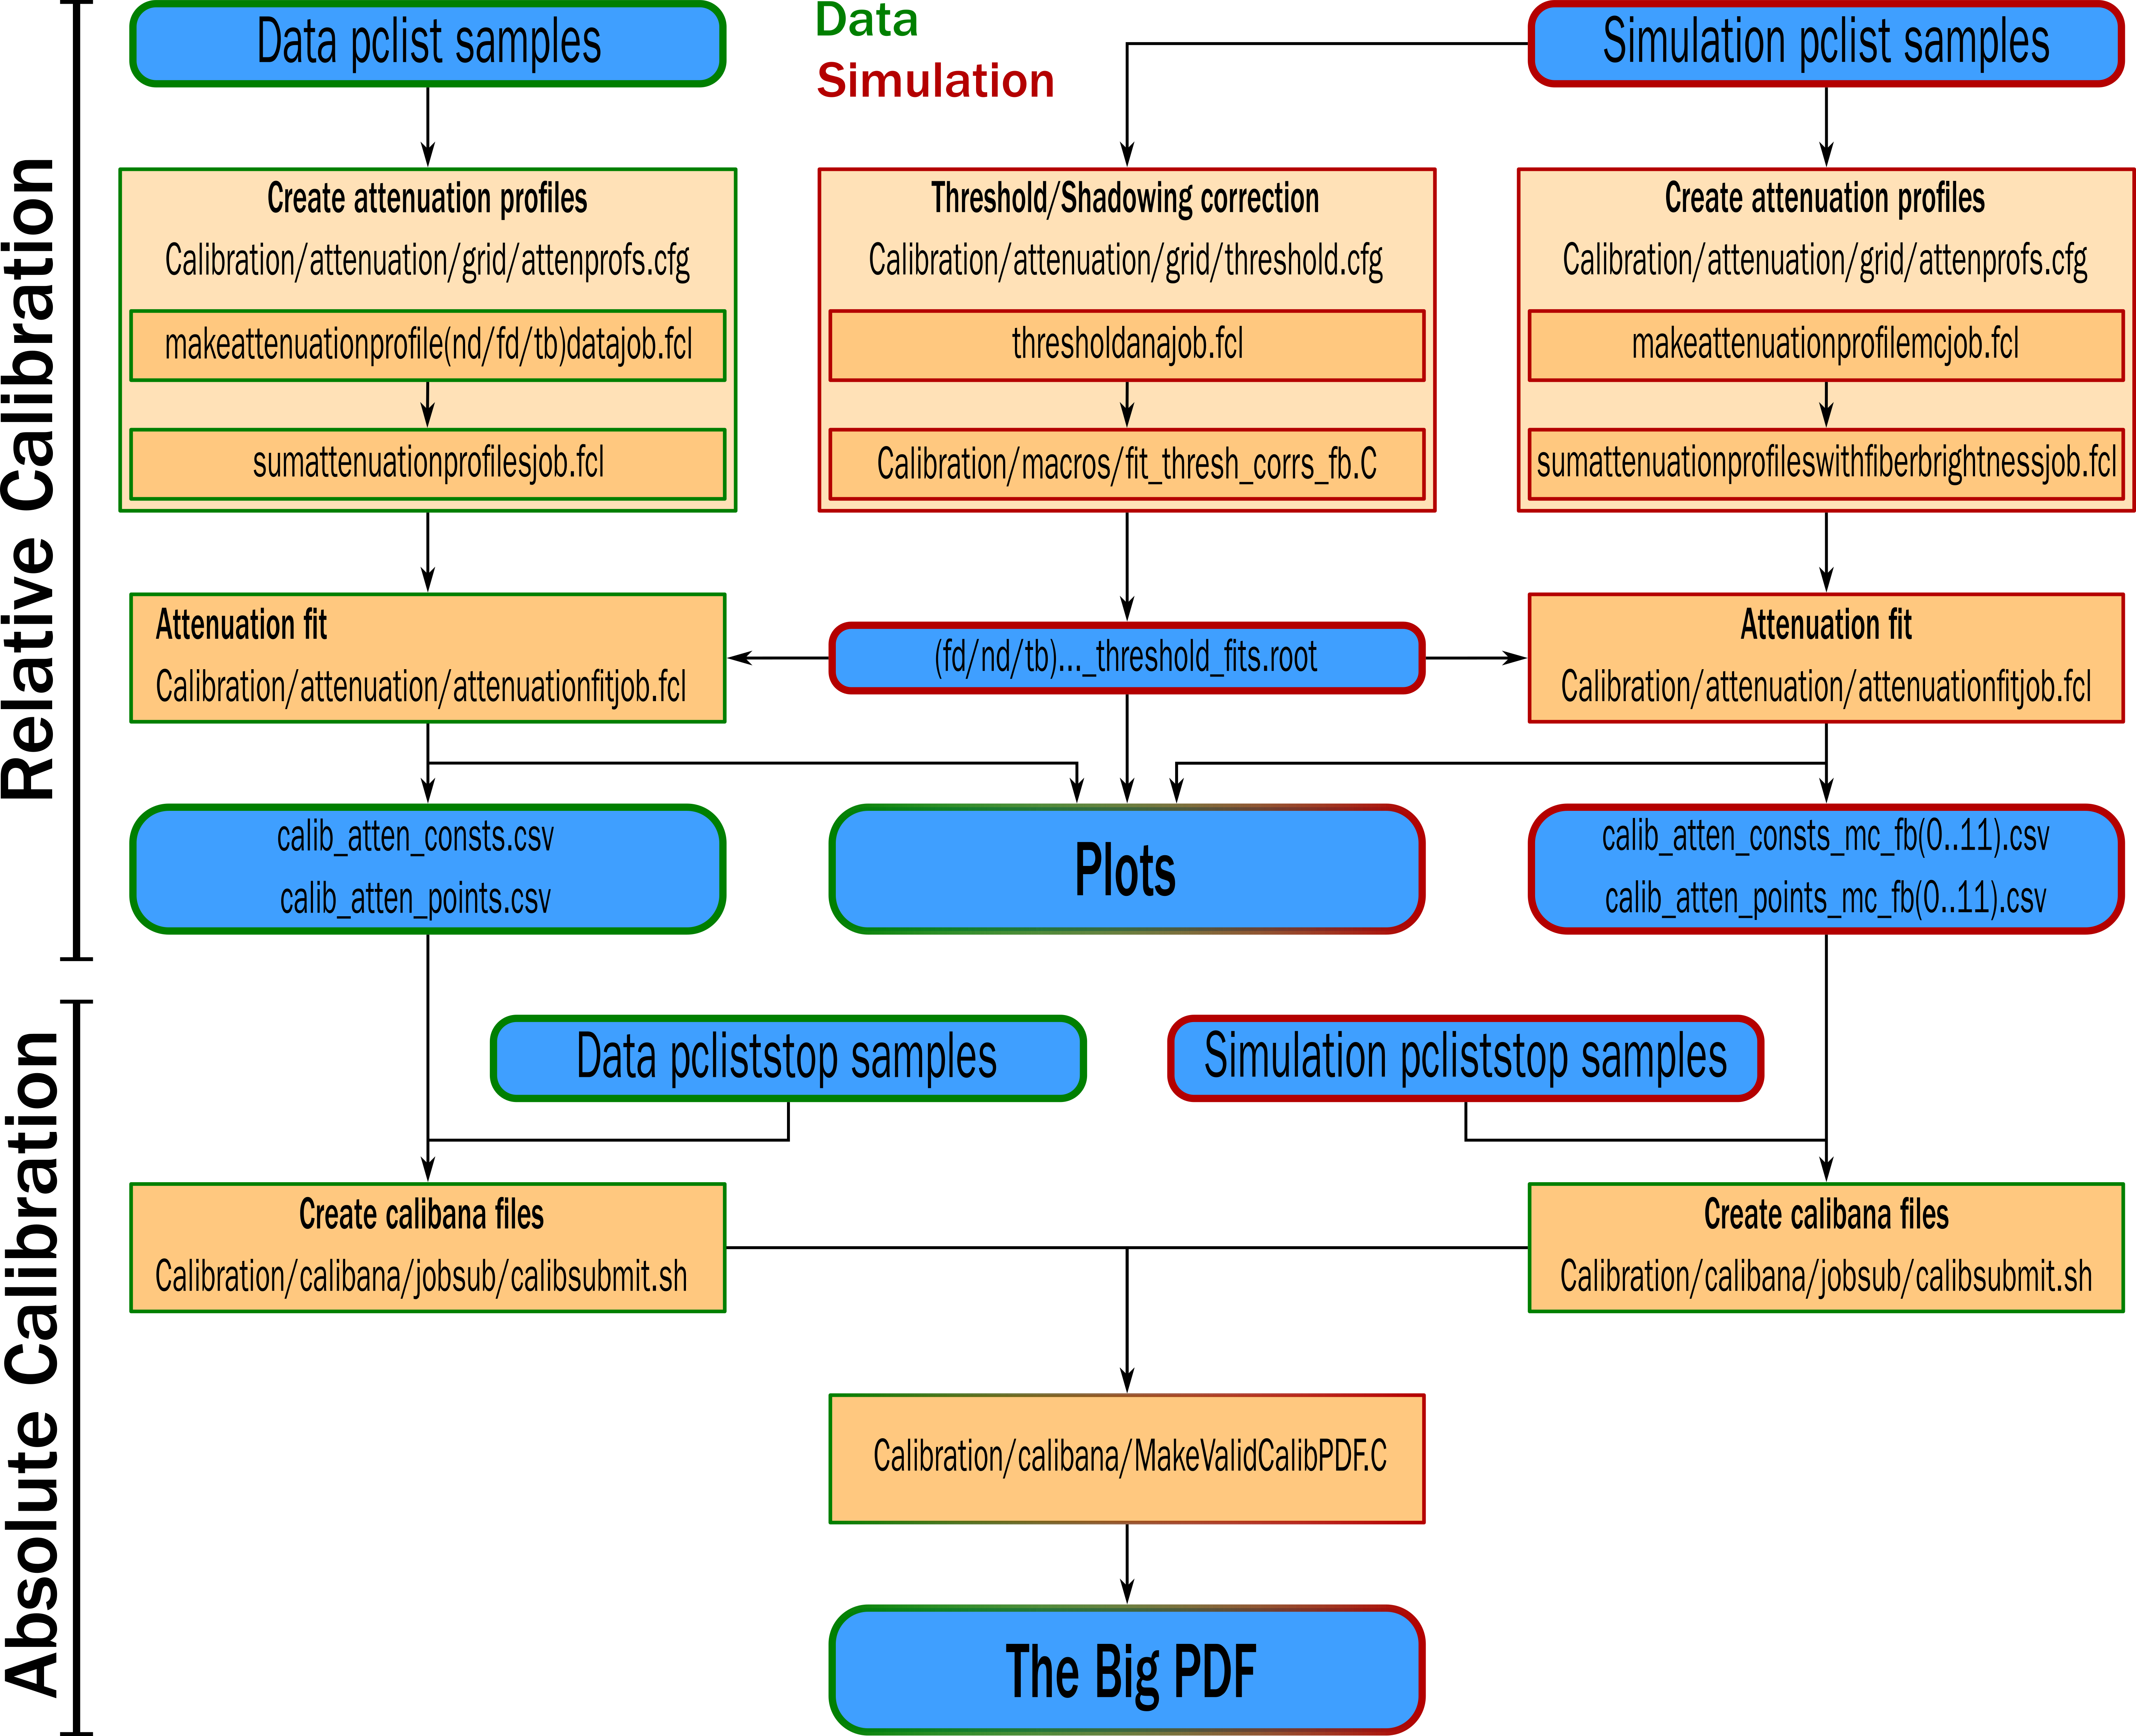
\includegraphics[width=\textwidth]{Plots/CalibrationFlowChart.png}
\caption{Flow chart showing the jobs and files needed for the NOvA calibration.}
\end{figure}

\subsection{Calibration uncertainties}

\section{NOvA Test Beam detector calibration}
\subsection{Overview}
History of TB calibration. What led to the final version of TB calibration. What can be done next.

\subsection{Test Beam data and simulation}

Dates and times when the data taking occured.

Period naming, possibly epochs (for P3).
List of data samples, plus MC samples that were used and pointer to the data-based simulation technote.
%Possibly refer to https://cdcvs.fnal.gov/redmine/projects/novatestbeam/wiki/Period_and_Epoch_Naming

Specific running conditions:
Underfilled cells
Faulty FEBs (Period 2 and Period 3)
Why do we do the calibration generally and why do we need to do in for Test Beam specifically

Temperature study (small overview)

\subsubsection{Definitions}
List all final data and simulation definitions used.

\subsection{Detector Brightness}

\begin{figure}[hbtp]
\centering
\begin{subfigure}[b]{0.495\textwidth}
\centering
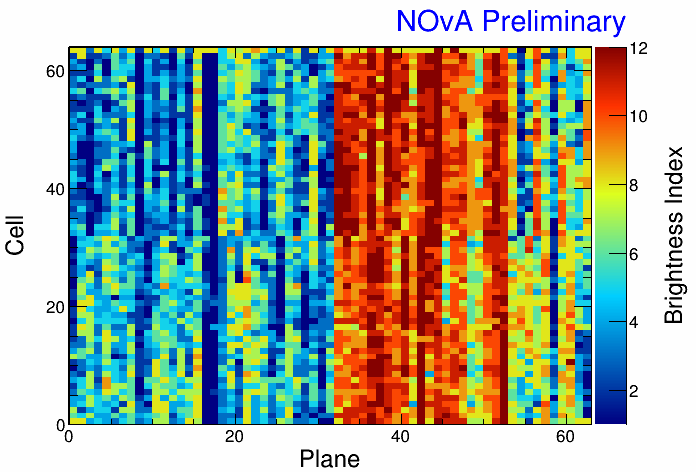
\includegraphics[width=\textwidth]{Plots/BrightnessIndex.png}
\end{subfigure}
%\hfill
\begin{subfigure}[b]{0.495\textwidth}
\centering
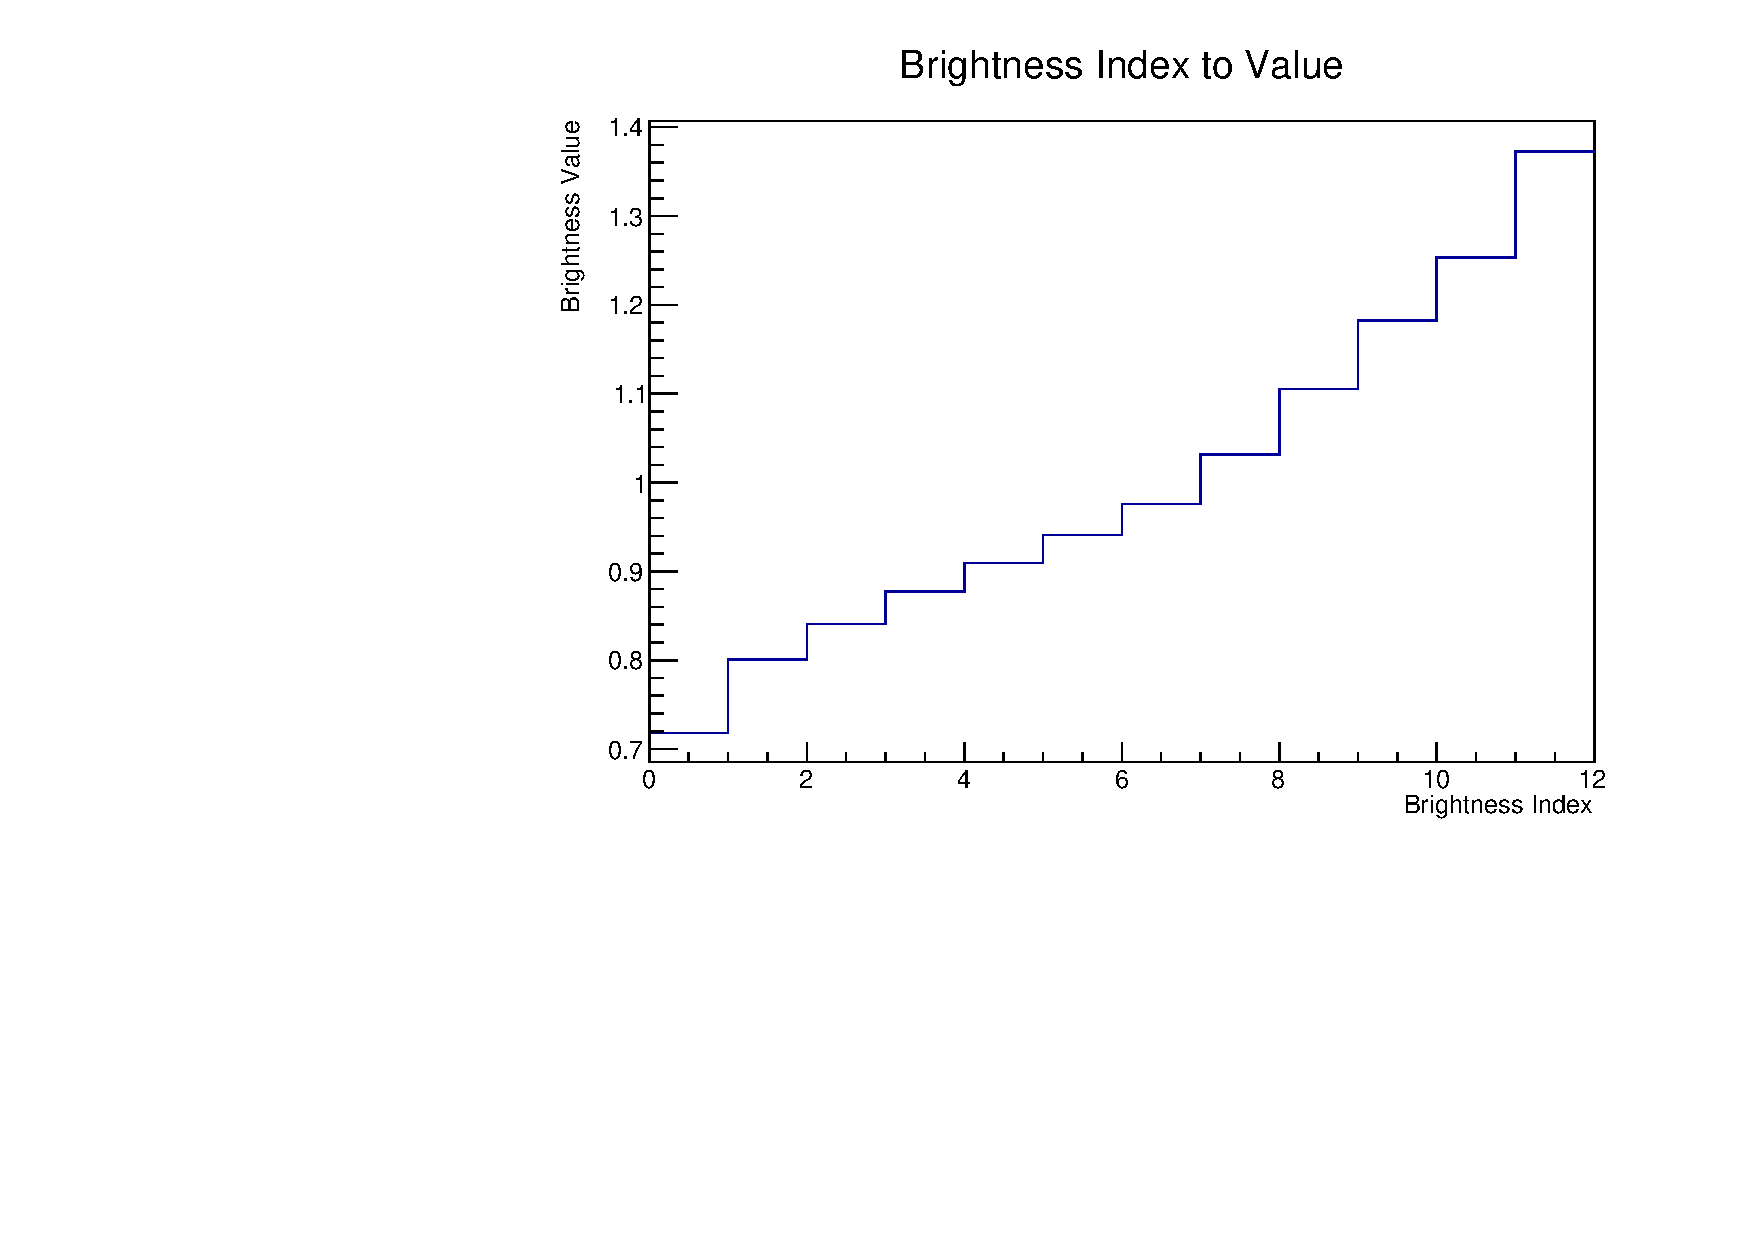
\includegraphics[width=\textwidth]{Plots/BrightnessIndexToValue.pdf}
\end{subfigure}
\caption{Brightness map}
\end{figure}



\subsection{Period 1}
Only a month of data, only first half of detector filled, primary/secondary beam halo, or oversaturation leading to FEB shutoffs [docdb:38349 and 41331].
Only used for comissioning, not used for any data analysis or calibration.

\subsection{Period 2}
What was done for the period 2 tb calibration, short overview of what has been done: test beam data were calibrated all at the same time without splitting them to separate epochs. We originally used Teresa's calibration MC sample, but after we saw disagreement, we developed a new MC based off of the period 3 data, which we ended up using for both period 2 and period 3. For fibre brightness we are also using the same MC from period 3 data as it represents the detector in its best condition.

\begin{figure}[hbtp]
\centering
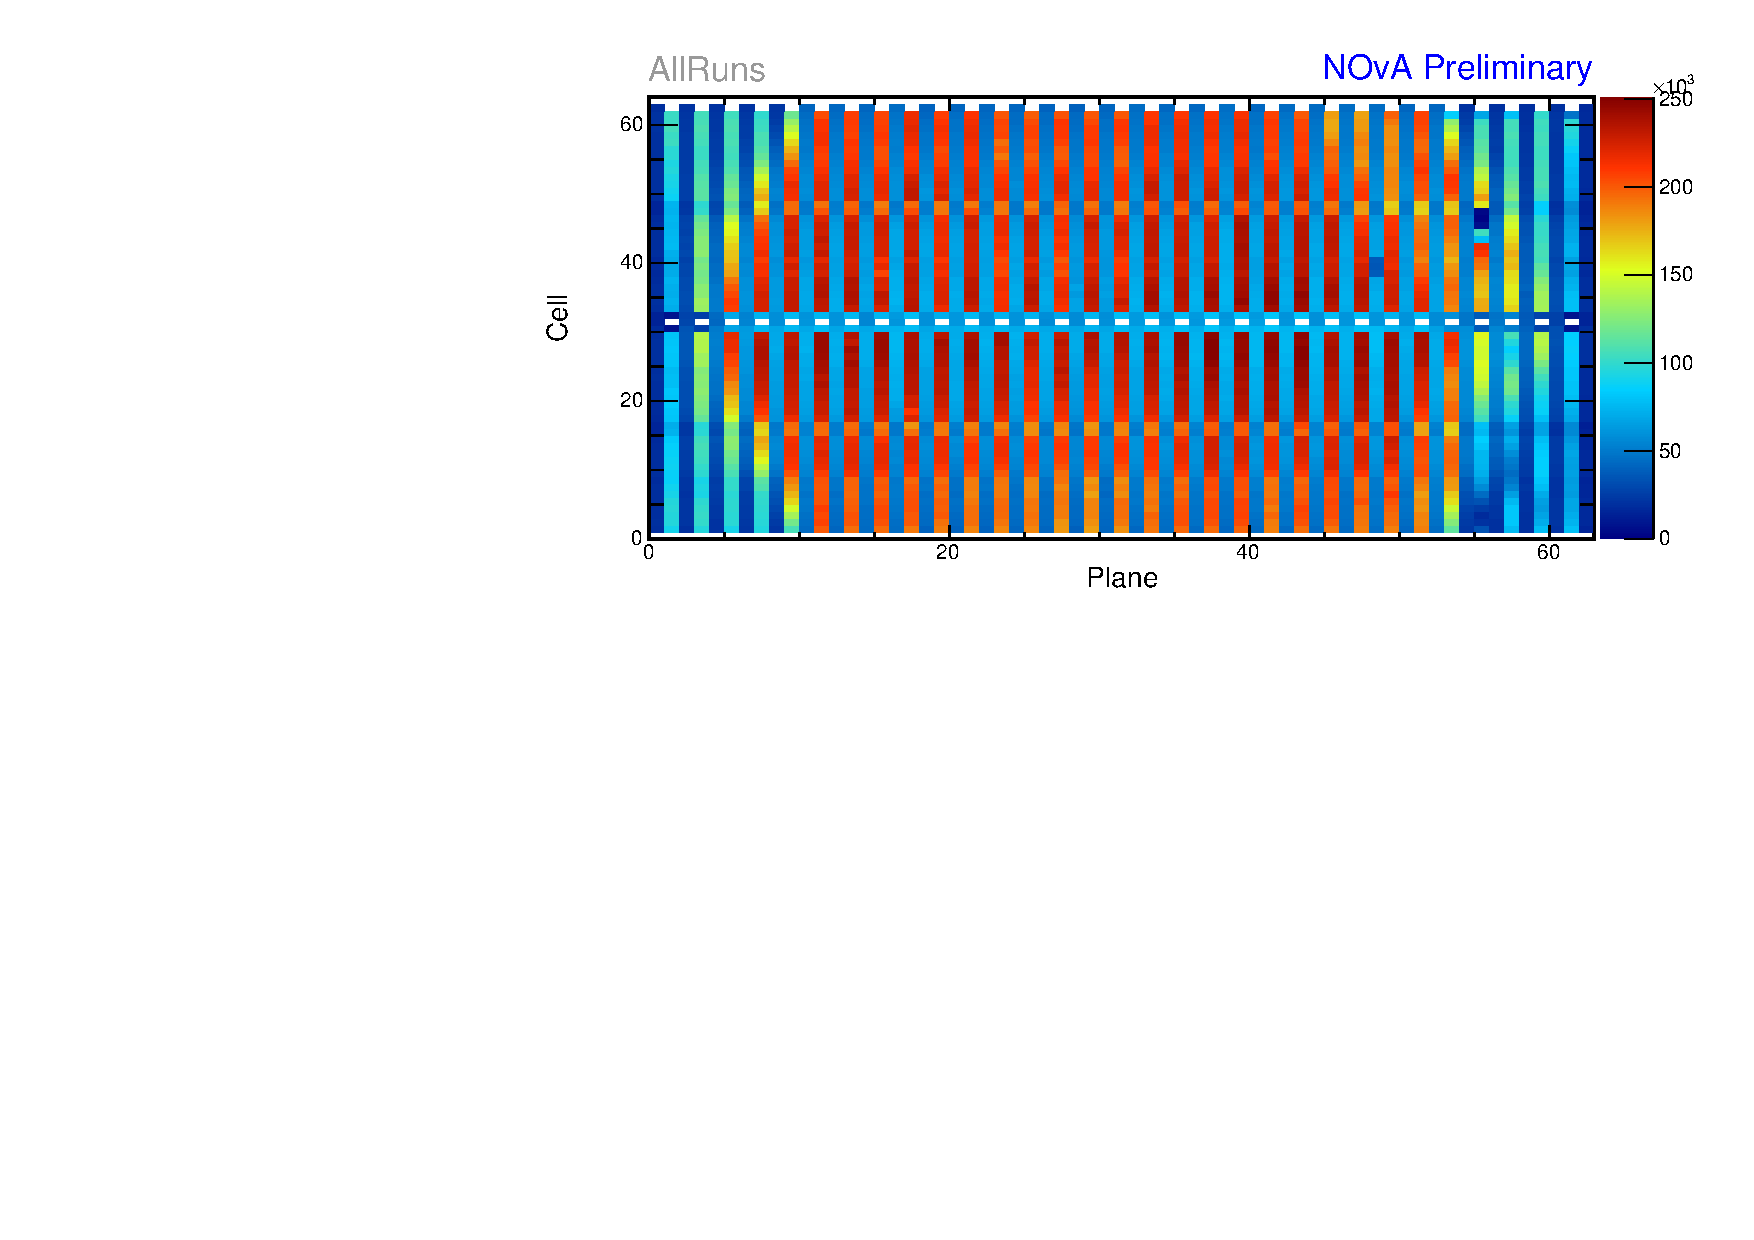
\includegraphics[width=\textwidth]{Plots/Attenprofs_P2Data_CellPlane_AllRuns.pdf}
\caption{Brightness map}
\end{figure}

\begin{figure}[hbtp]
\centering
\begin{subfigure}[b]{\textwidth}
\centering
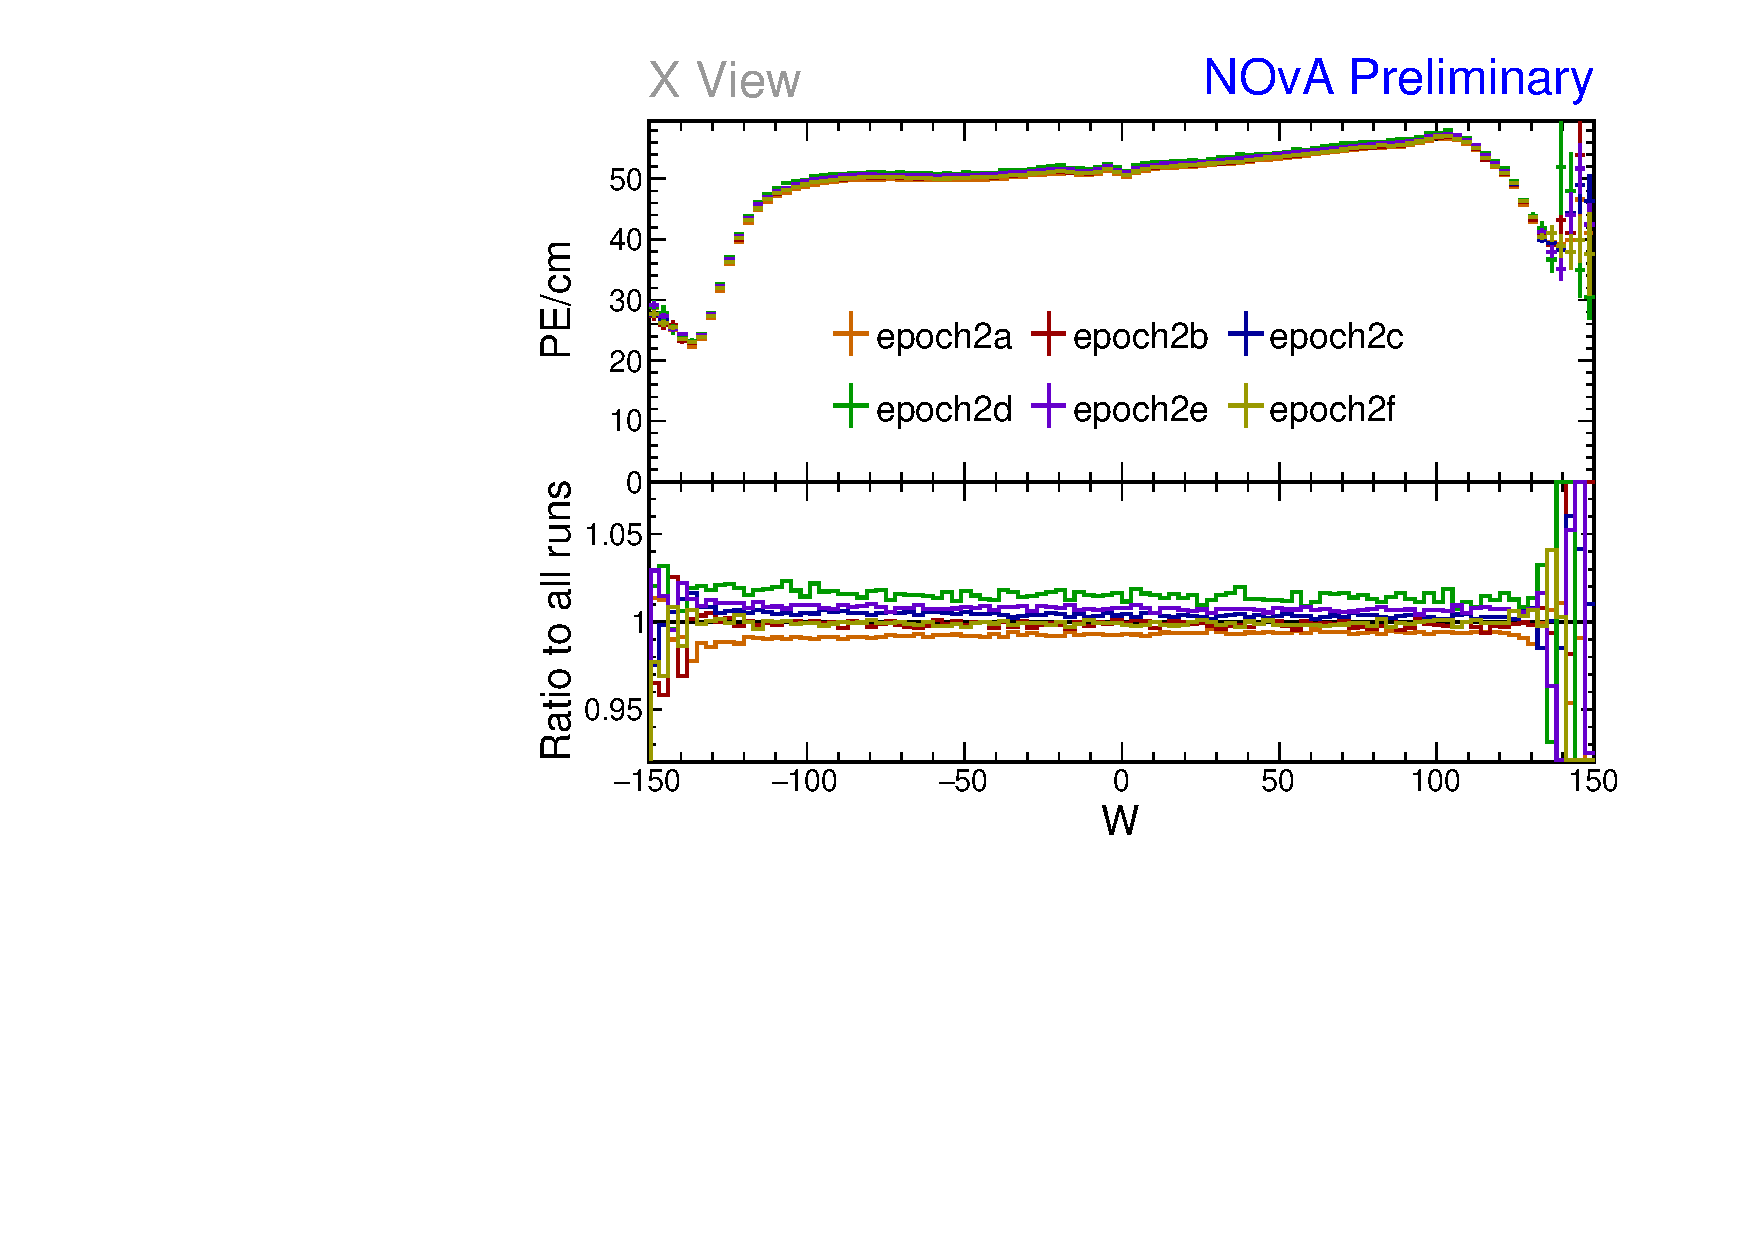
\includegraphics[width=\textwidth]{Plots/Attenprofs_P2Data_WPE_corr_xy_X_Combined.pdf}
\end{subfigure}
\begin{subfigure}[b]{\textwidth}
\centering
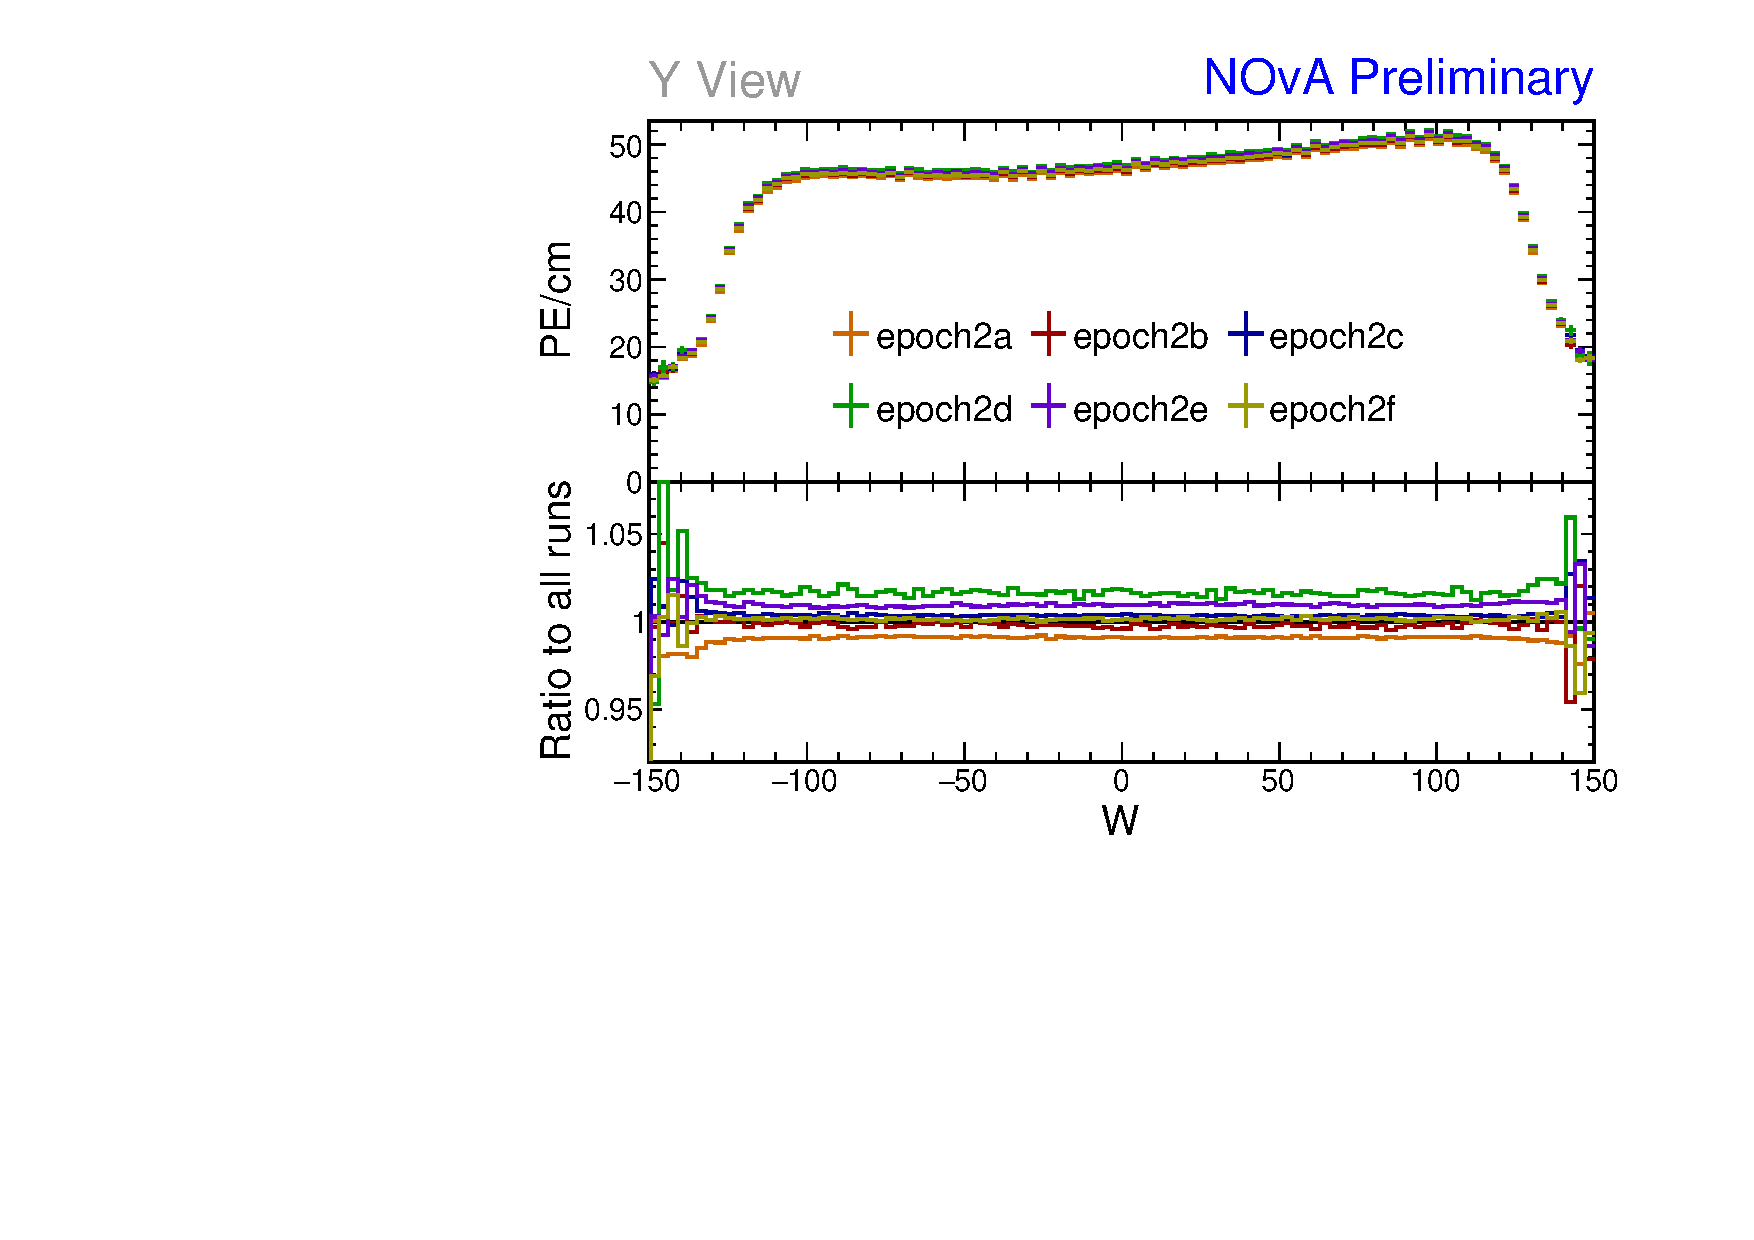
\includegraphics[width=\textwidth]{Plots/Attenprofs_P2Data_WPE_corr_xy_Y_Combined.pdf}
\end{subfigure}
\caption{Brightness map}
\end{figure}

\begin{figure}[hbtp]
\centering
\begin{subfigure}[b]{\textwidth}
\centering
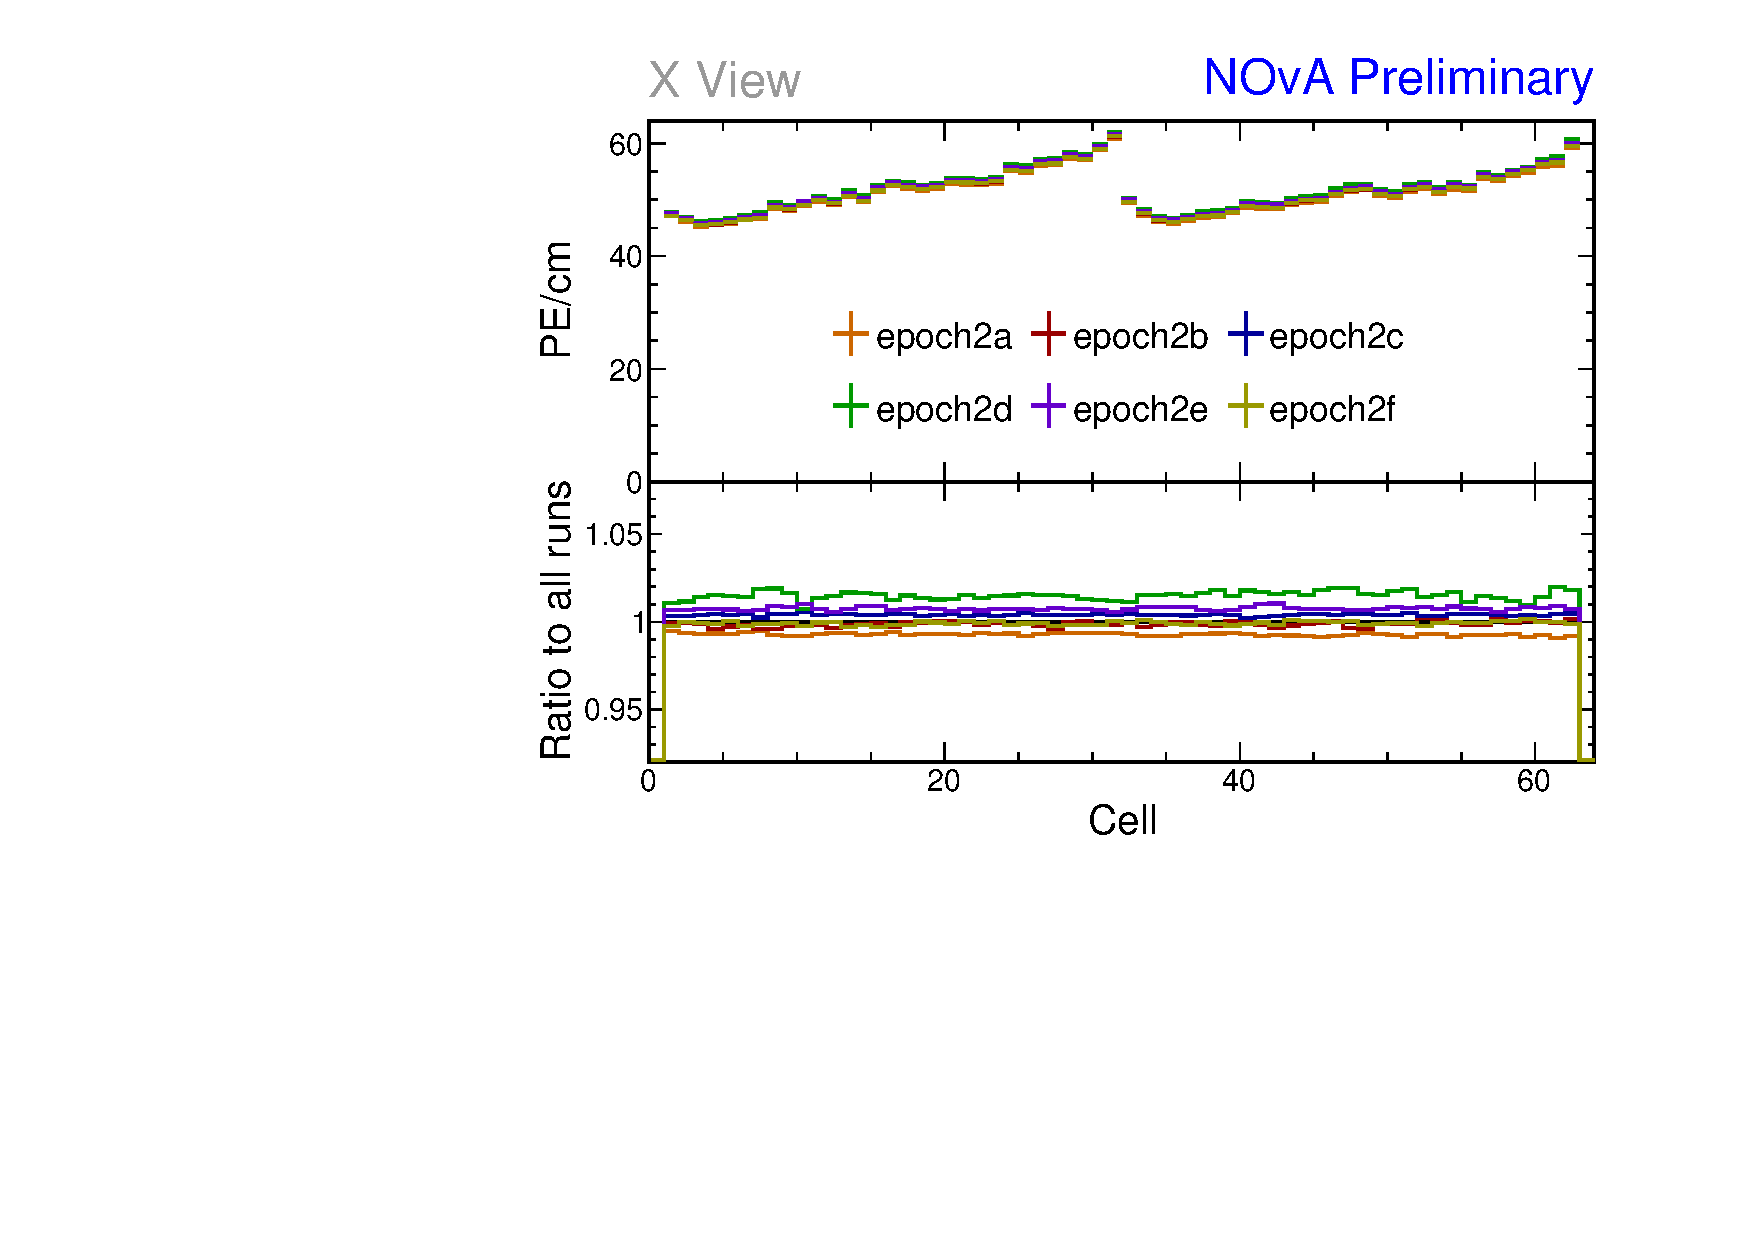
\includegraphics[width=\textwidth]{Plots/Attenprofs_P2Data_CellPE_X_Combined.pdf}
\end{subfigure}
\begin{subfigure}[b]{\textwidth}
\centering
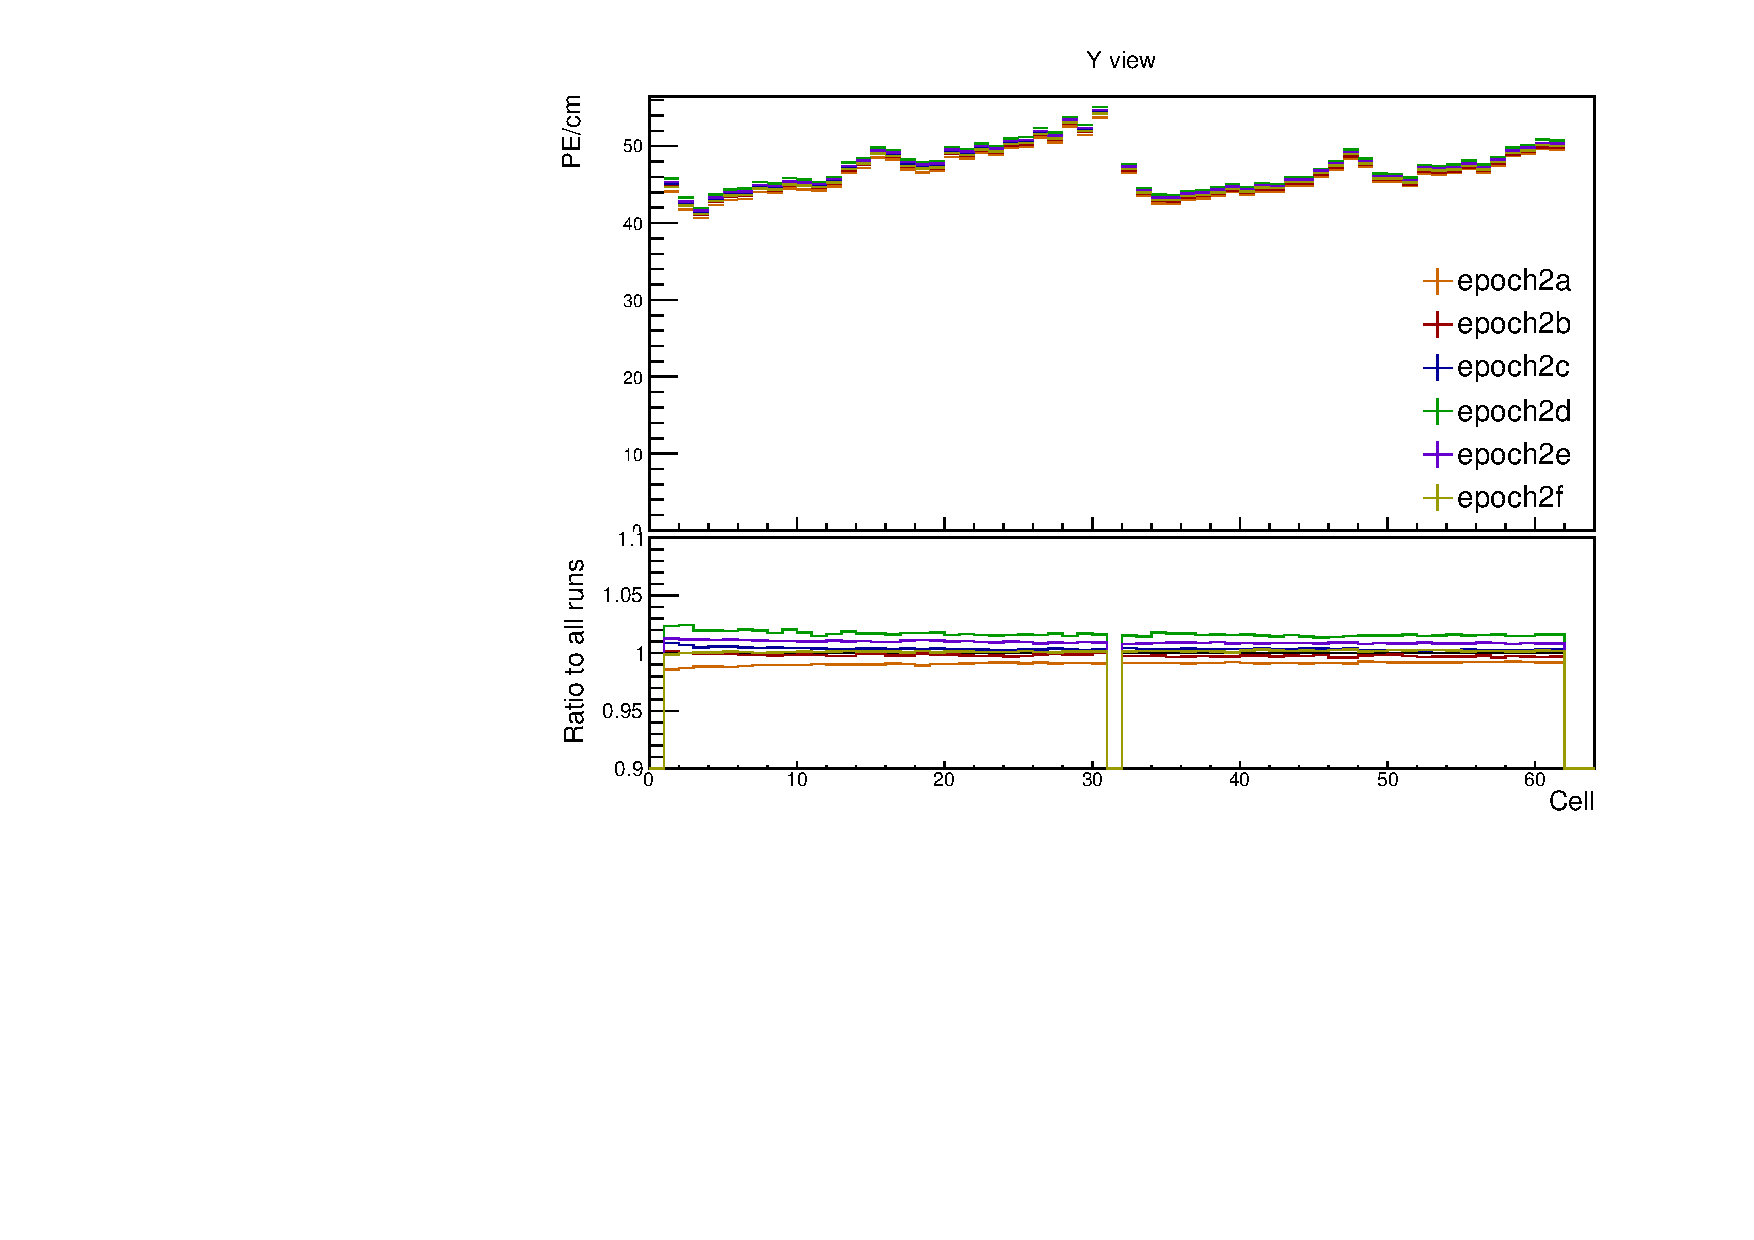
\includegraphics[width=\textwidth]{Plots/Attenprofs_P2Data_CellPE_Y_Combined.pdf}
\end{subfigure}
\caption{Brightness map}
\end{figure}

\begin{figure}[hbtp]
\centering
\begin{subfigure}[b]{\textwidth}
\centering
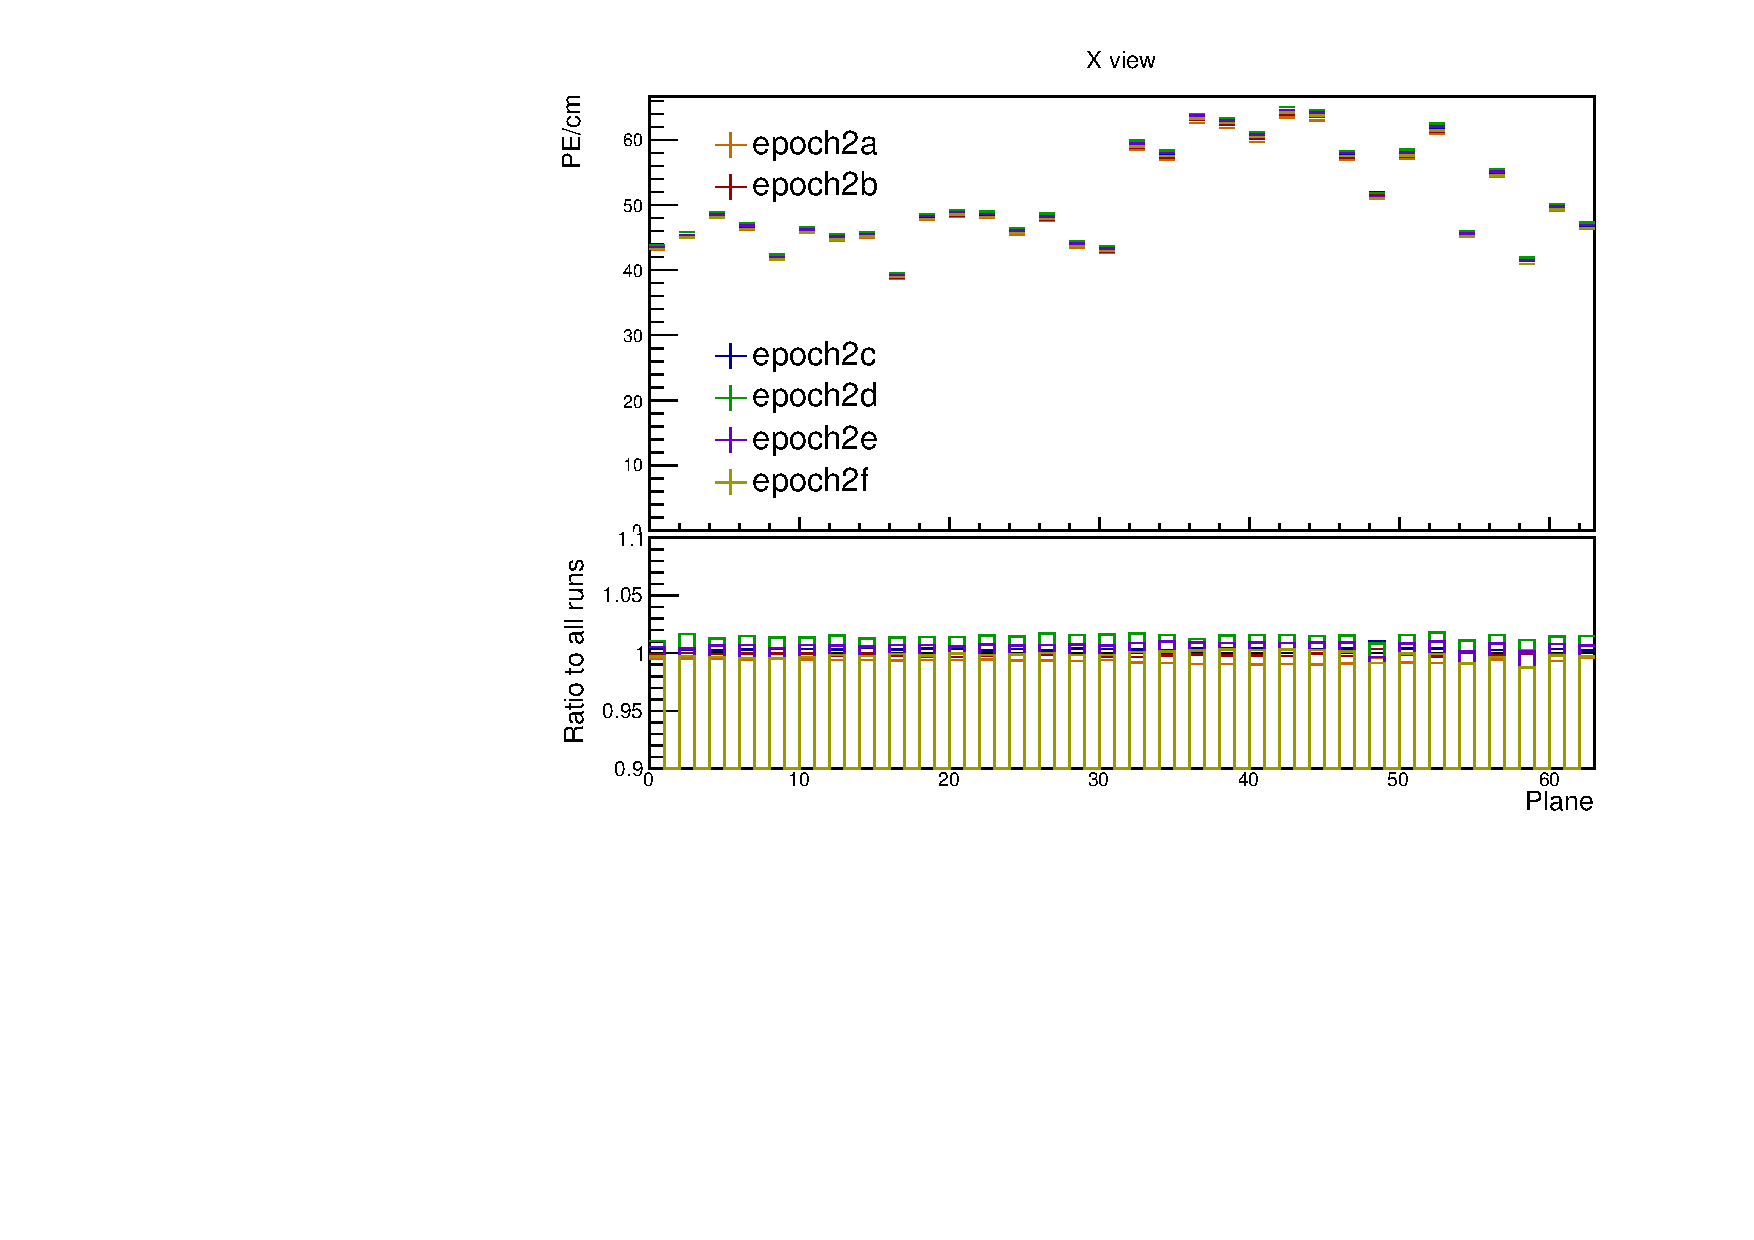
\includegraphics[width=\textwidth]{Plots/Attenprofs_P2Data_PlanePE_X_Combined.pdf}
\end{subfigure}
\begin{subfigure}[b]{\textwidth}
\centering
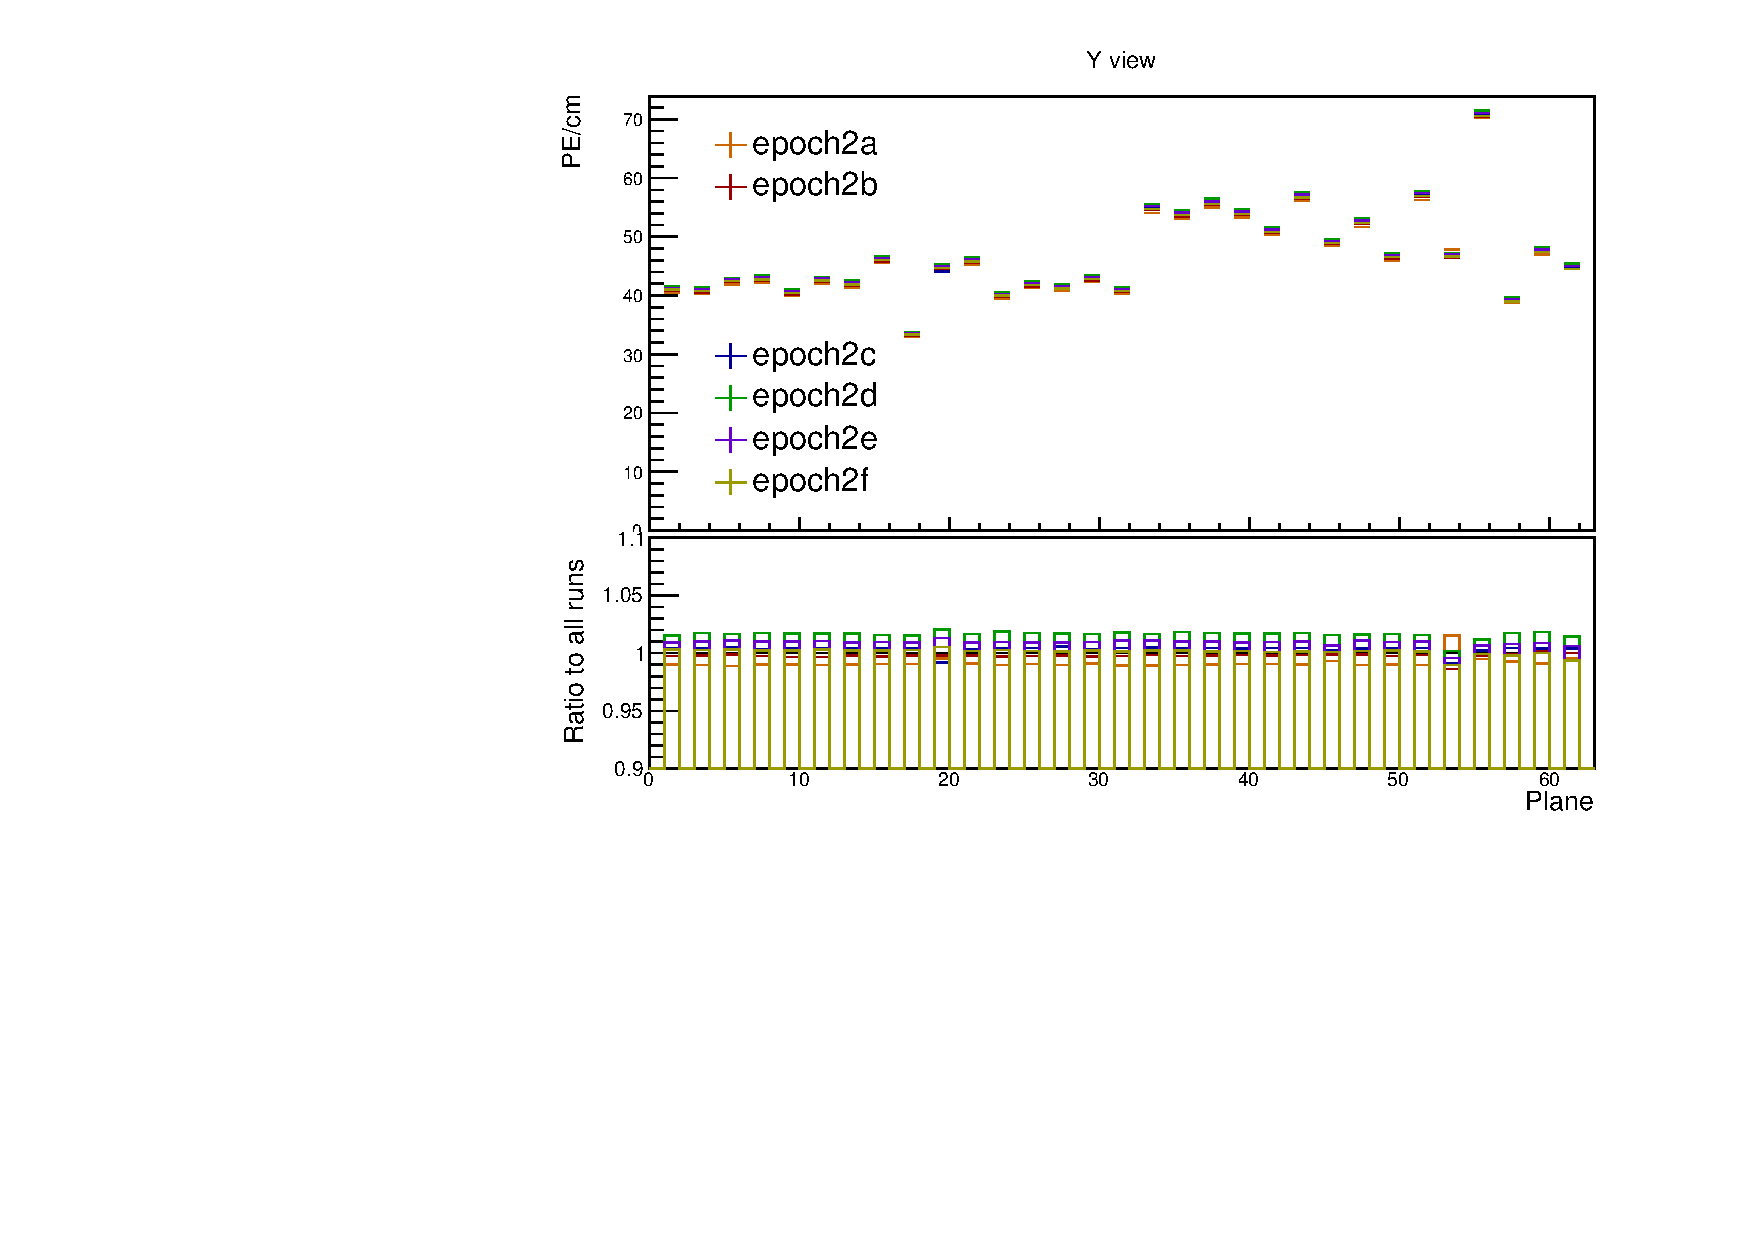
\includegraphics[width=\textwidth]{Plots/Attenprofs_P2Data_PlanePE_Y_Combined.pdf}
\end{subfigure}
\caption{Brightness map}
\end{figure}

\subsection{Period 3}
Separation of Period 3 data into different epochs based on the running conditions (include plot of the running conditions). We are separating data into pre- and post- filling states. We're using only the fully-refilled post-FEB swap data from period 3 as a basis for the simulation creation.

\subsubsection{Period 4}


\subsection{Simulation}
We used a data-based simulation of cosmic muons for the Test Beam detector calibration. The details are described in the technote XXX. We used this and this data as a basis and this and this data for the fiber brighness file.

Should I put this into a separate Appendix (or just a stand alone technote) as well?
First we needed to select the right data that could serve as a basis for the simulation. Comparing this with the previous version and how did the totlength cut change our cuts. Why do we need to remove the beam events and how do we remove them (CosZ<0.98). Include plots showing some distributions and how they are affected by the cuts. How many events do we have after the cuts?

\subsection{Relative calibration}

Attenutation profiles have a constant binnin fNBins=100 (in w), same for ND, FD and TB. This results in an effectively finer binning for TB compared to ND and FD. For FD w = (-900,+900), ND: (-250,+250), TB: (-150,+150).
TB: 3cm/bin, ND: 5cm/bin, FD: 18cm/bin.
What effect could this have on the relative calibration results? Particularly on the calibration shape?

\subsection{Results}
Table of final results.
Final CSVs are locate in the \path{/nova/ana/testbeam/calibration} and they have been included in the vXX.XX calibration tag.

Plots of absolute calibration results

\subsection{Validation}
Comparisons with older version of calibration and maybe with the FD and ND

\end{document}